\documentclass{beamer}

\usetheme{metropolis}
\usepackage[default]{raleway}

\usepackage{booktabs}

\setbeamertemplate{footline}{}

\title{%
    The where and why of cost variation in the National Health Service\\
    \small Understanding cost variation with machine learning
}

\author{%
    Henry Wilde\\
    \scriptsize{%
        \textit{Supervised by:} Dr Jonathan Gillard and Dr Vincent Knight
    }
}

\institute{%
    \vfill%
    \centering%
    
\includegraphics[height=.2\paperheight]{./img/cu_logo.png}%
    \hspace{5pt}%
    
\includegraphics[height=.2\paperheight]{./img/cthb_logo.jpg}
}

\begin{document}

\frame{%
    \maketitle%
}

\frame{\frametitle{The data}
    \begin{itemize}
        \item The Cwm Taf University Health Board
        \item April 2012 through April 2017
        \item 2.4 million patient-episode records with 260 attributes
    \end{itemize}

    \begin{table}[htbp]
        \resizebox{\textwidth}{!}{%
            \begin{tabular}{lllrrlllr}
\toprule
&            &              &      Net Cost &   Age (years) &    HRG &
Admission Date &    Discharge Date &  Length of Stay (days) \\
PATIENT ID & SPELL ID & EPISODE ID &              &       &        &             &             &           \\
\midrule
ID\_123456 & M1001 & M1001-1 &   858.14 &  74 &  EA05Z &  2015-05-06 &  2015-05-06 &       0.0 \\
                   & M1211 & M1211-1 &   333.95 &  74 &  FZ38F &  2015-07-15 &  2015-08-01 &      17.0 \\
                   &            & M1211-2 &   706.09 &  74 &  FZ38F &  2015-07-15 &  2015-08-01 &      17.0 \\
                   &            & M1211-3 &  8671.31 &  74 &  RC16Z &  2015-07-15 &  2015-08-01 &      17.0 \\
\bottomrule
\end{tabular}

        }
    \end{table}
}

\section{Where does variation come from?}

\frame{\frametitle{Key attributes and what they look like}
    \begin{figure}
        \centering
        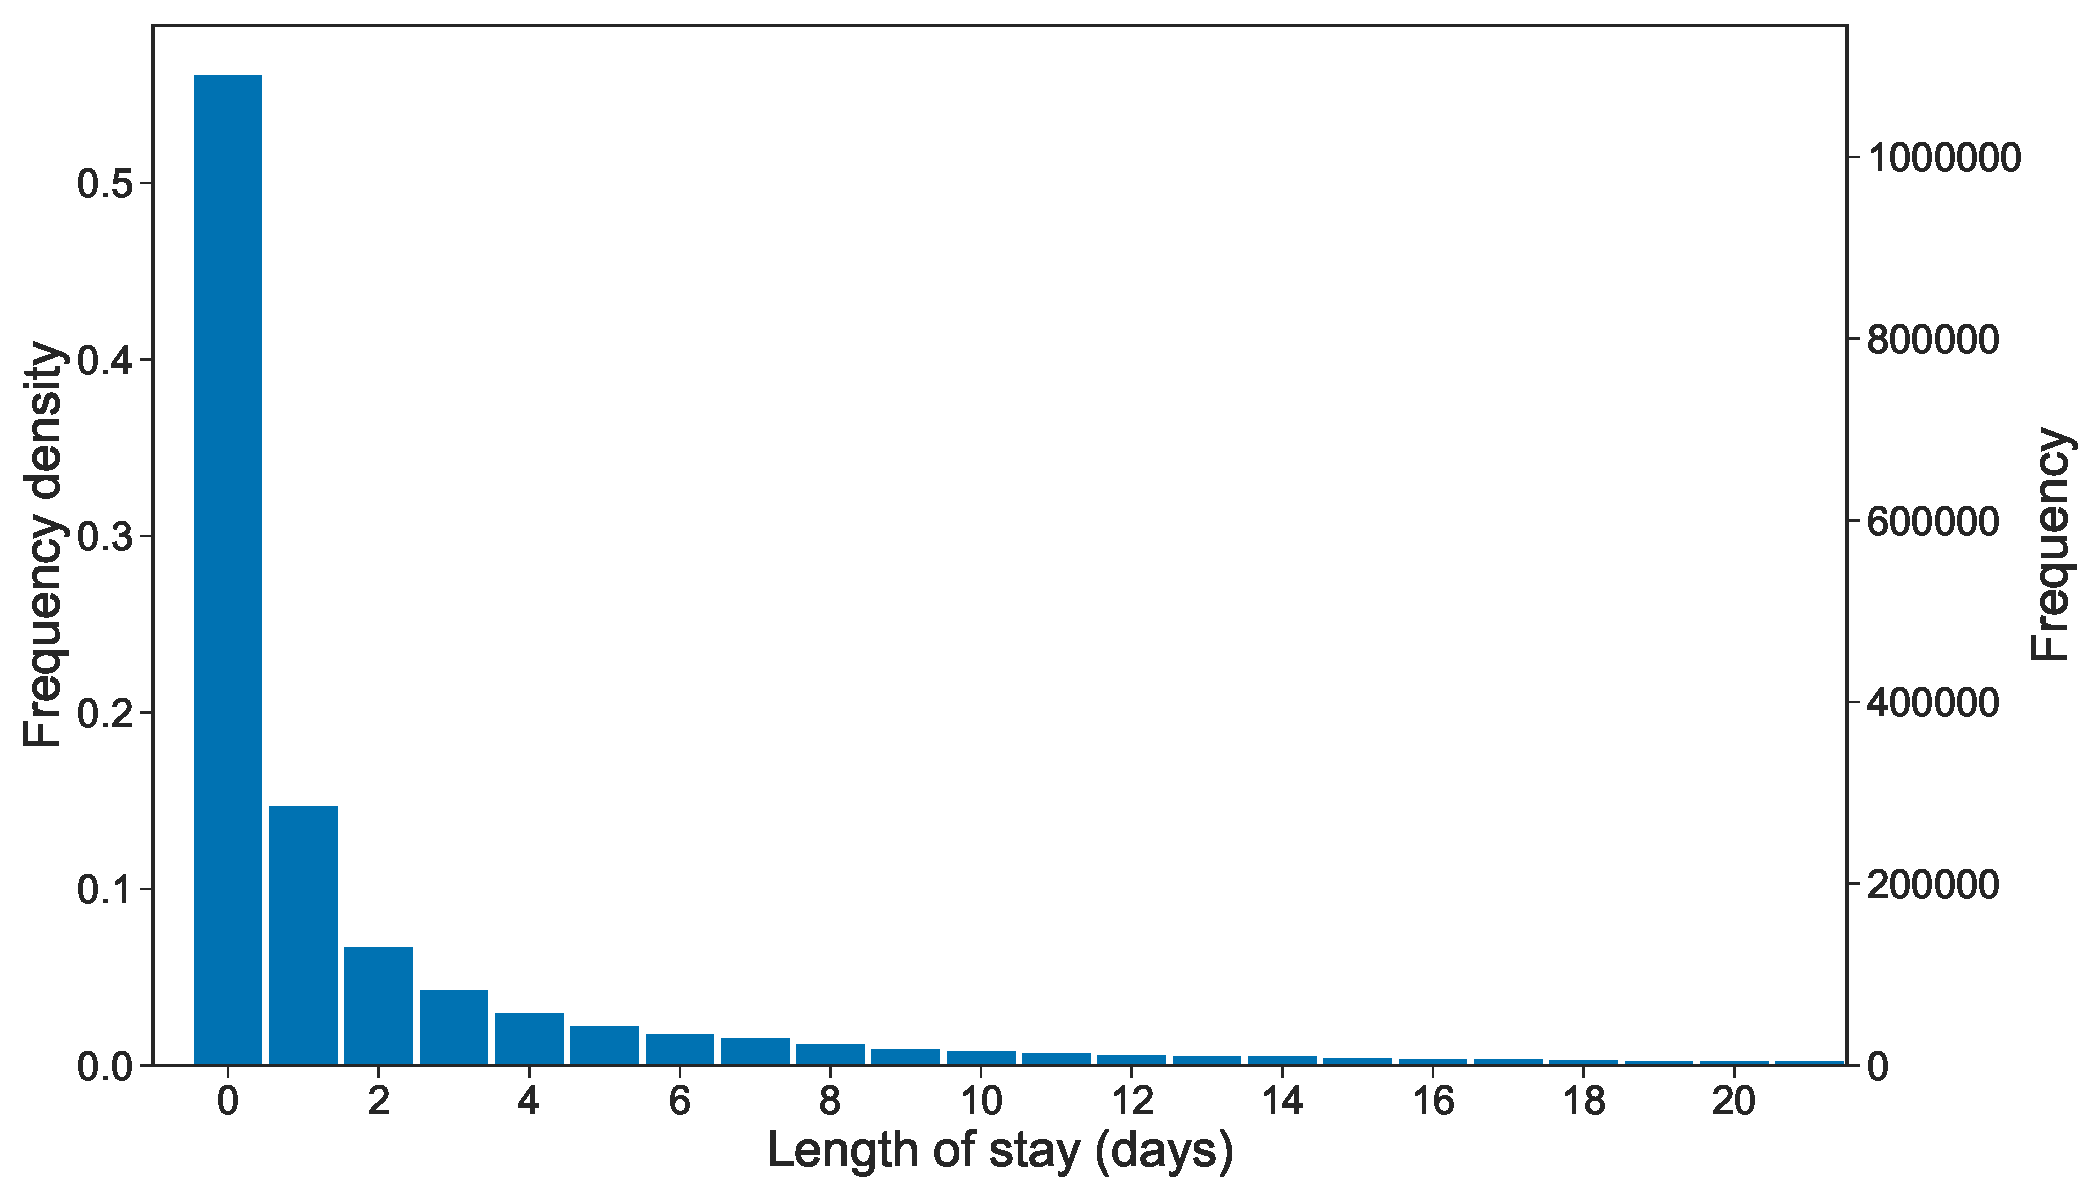
\includegraphics[width=.5\linewidth]{./img/los.pdf}

        \begin{minipage}{.5\linewidth}
            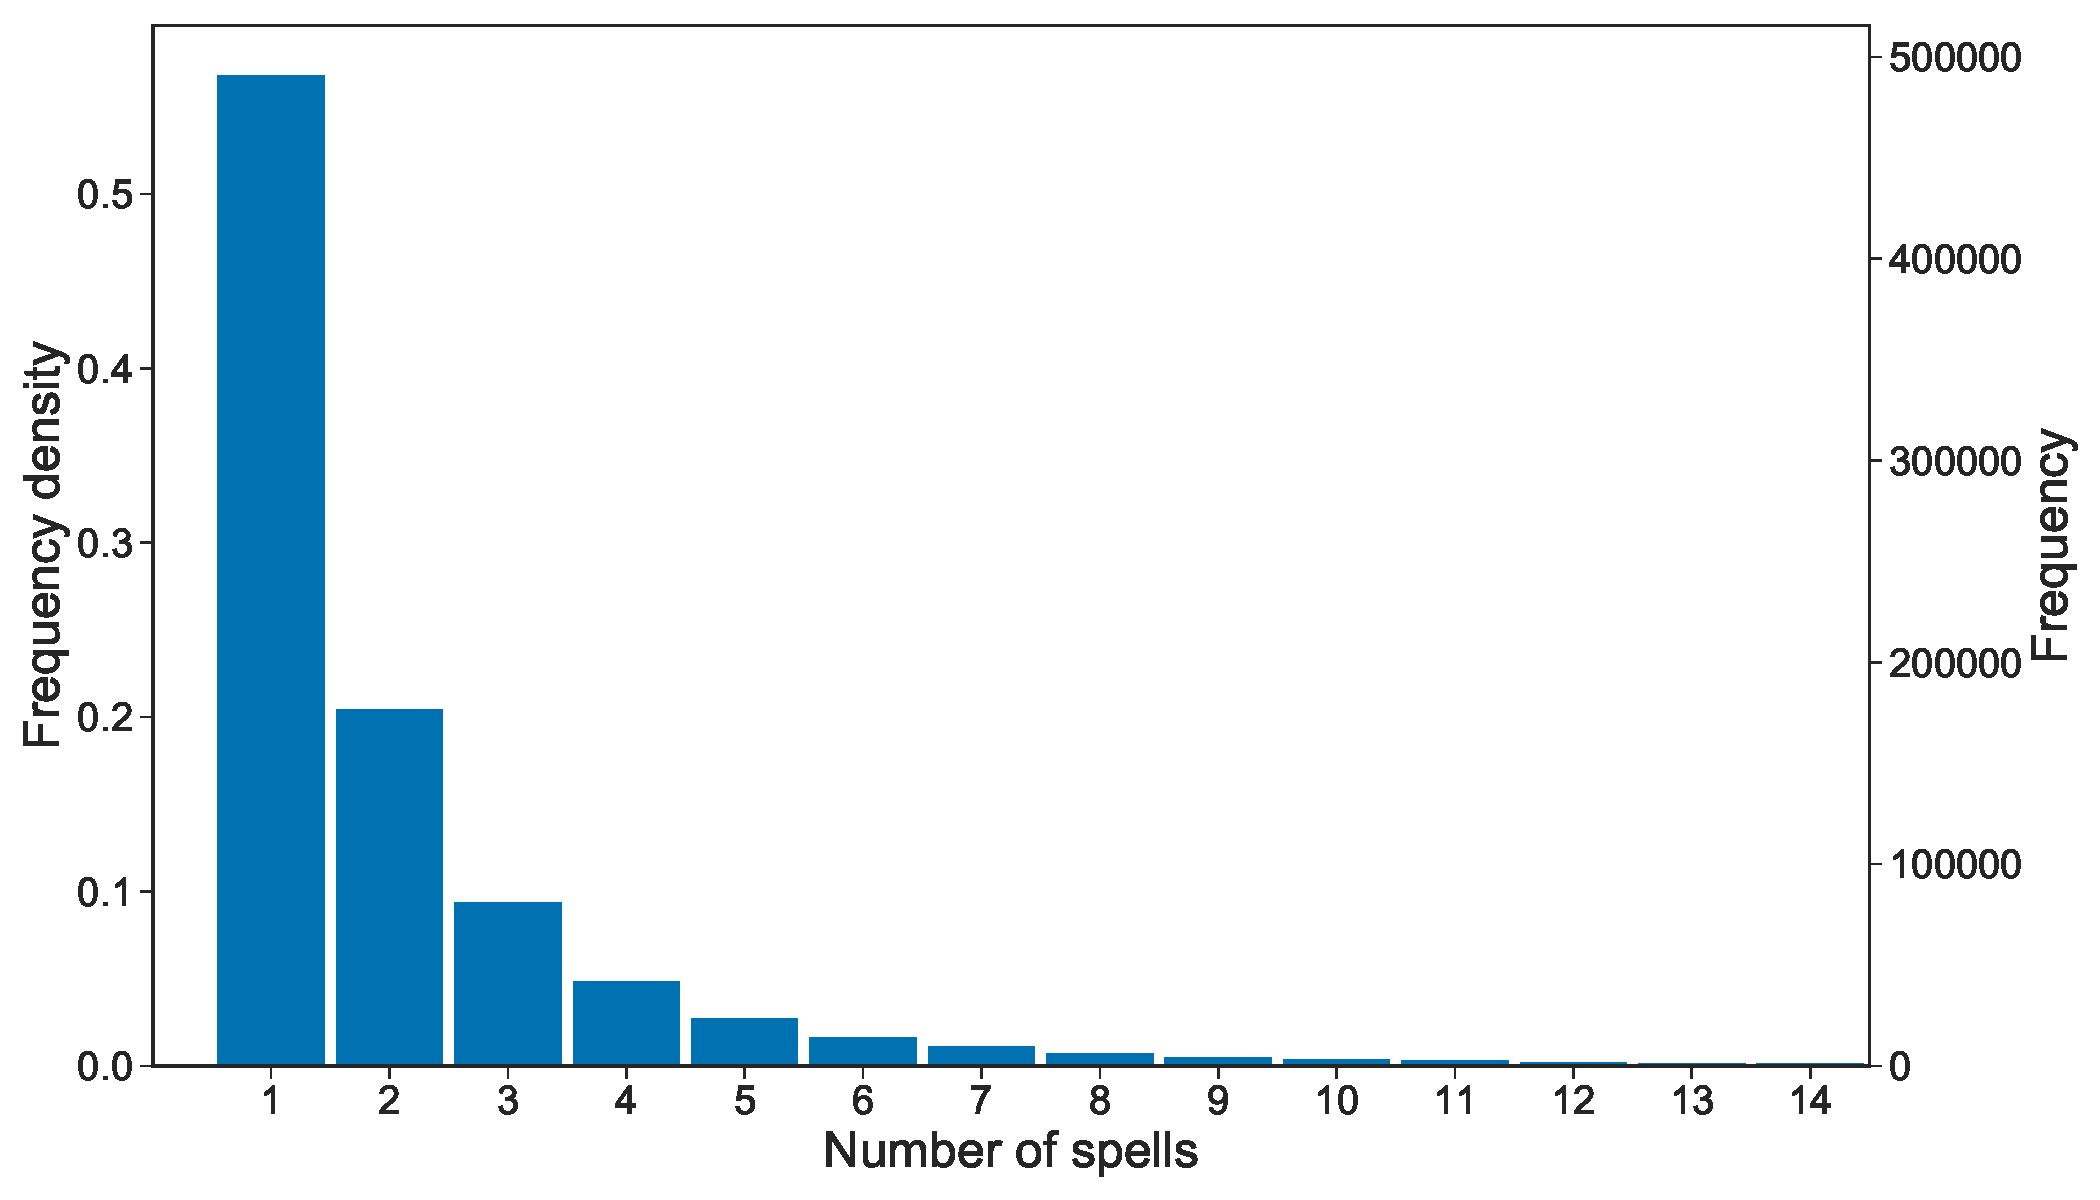
\includegraphics[width=\linewidth]{./img/spells.pdf}
        \end{minipage}%
        \hfill%
        \begin{minipage}{.5\linewidth}
            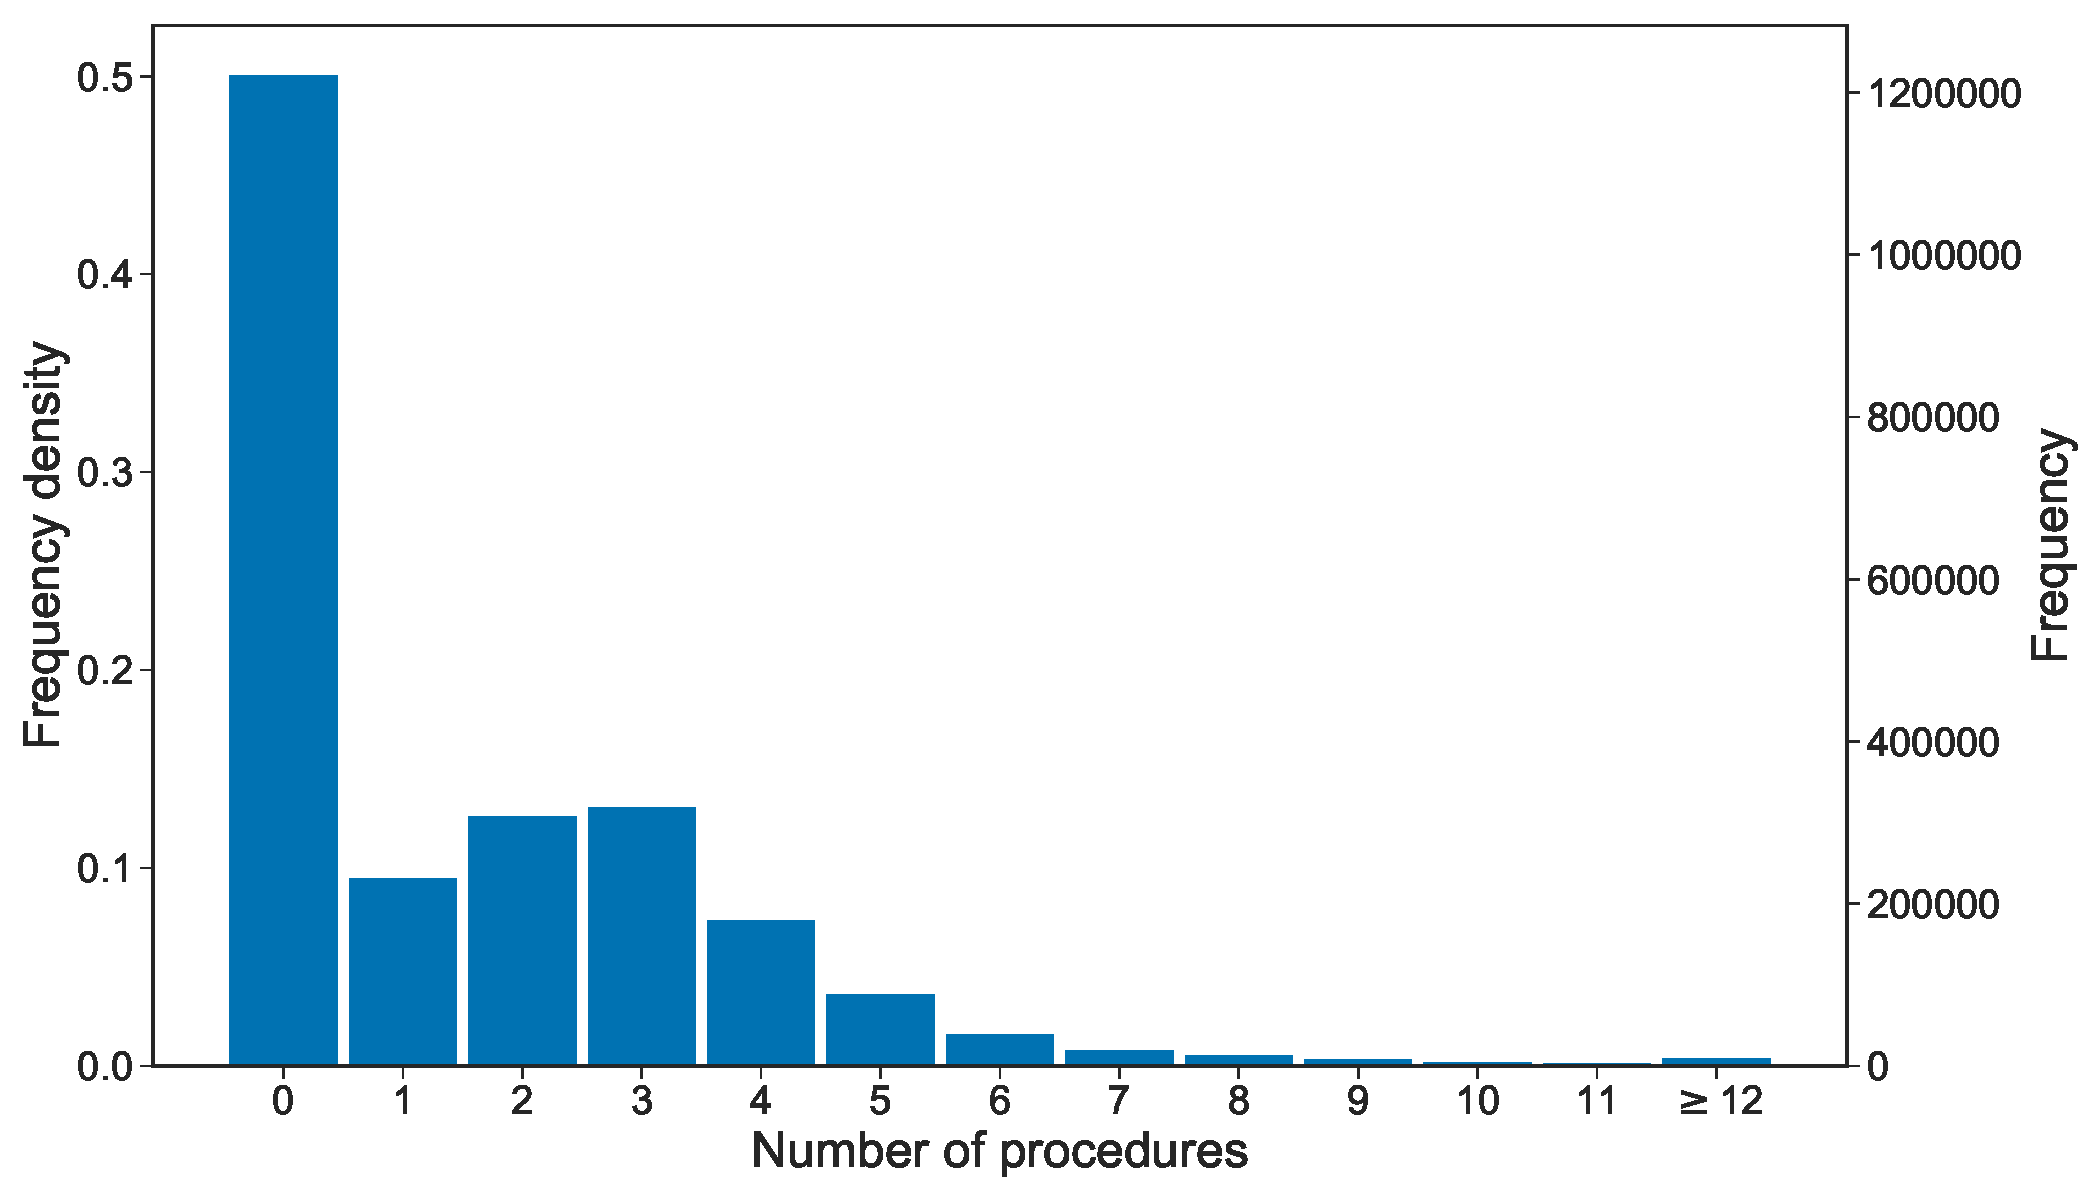
\includegraphics[width=\linewidth]{./img/proc.pdf}
        \end{minipage}
    \end{figure}
}

%\frame{\frametitle{Relative importance}
%    \begin{figure}
%        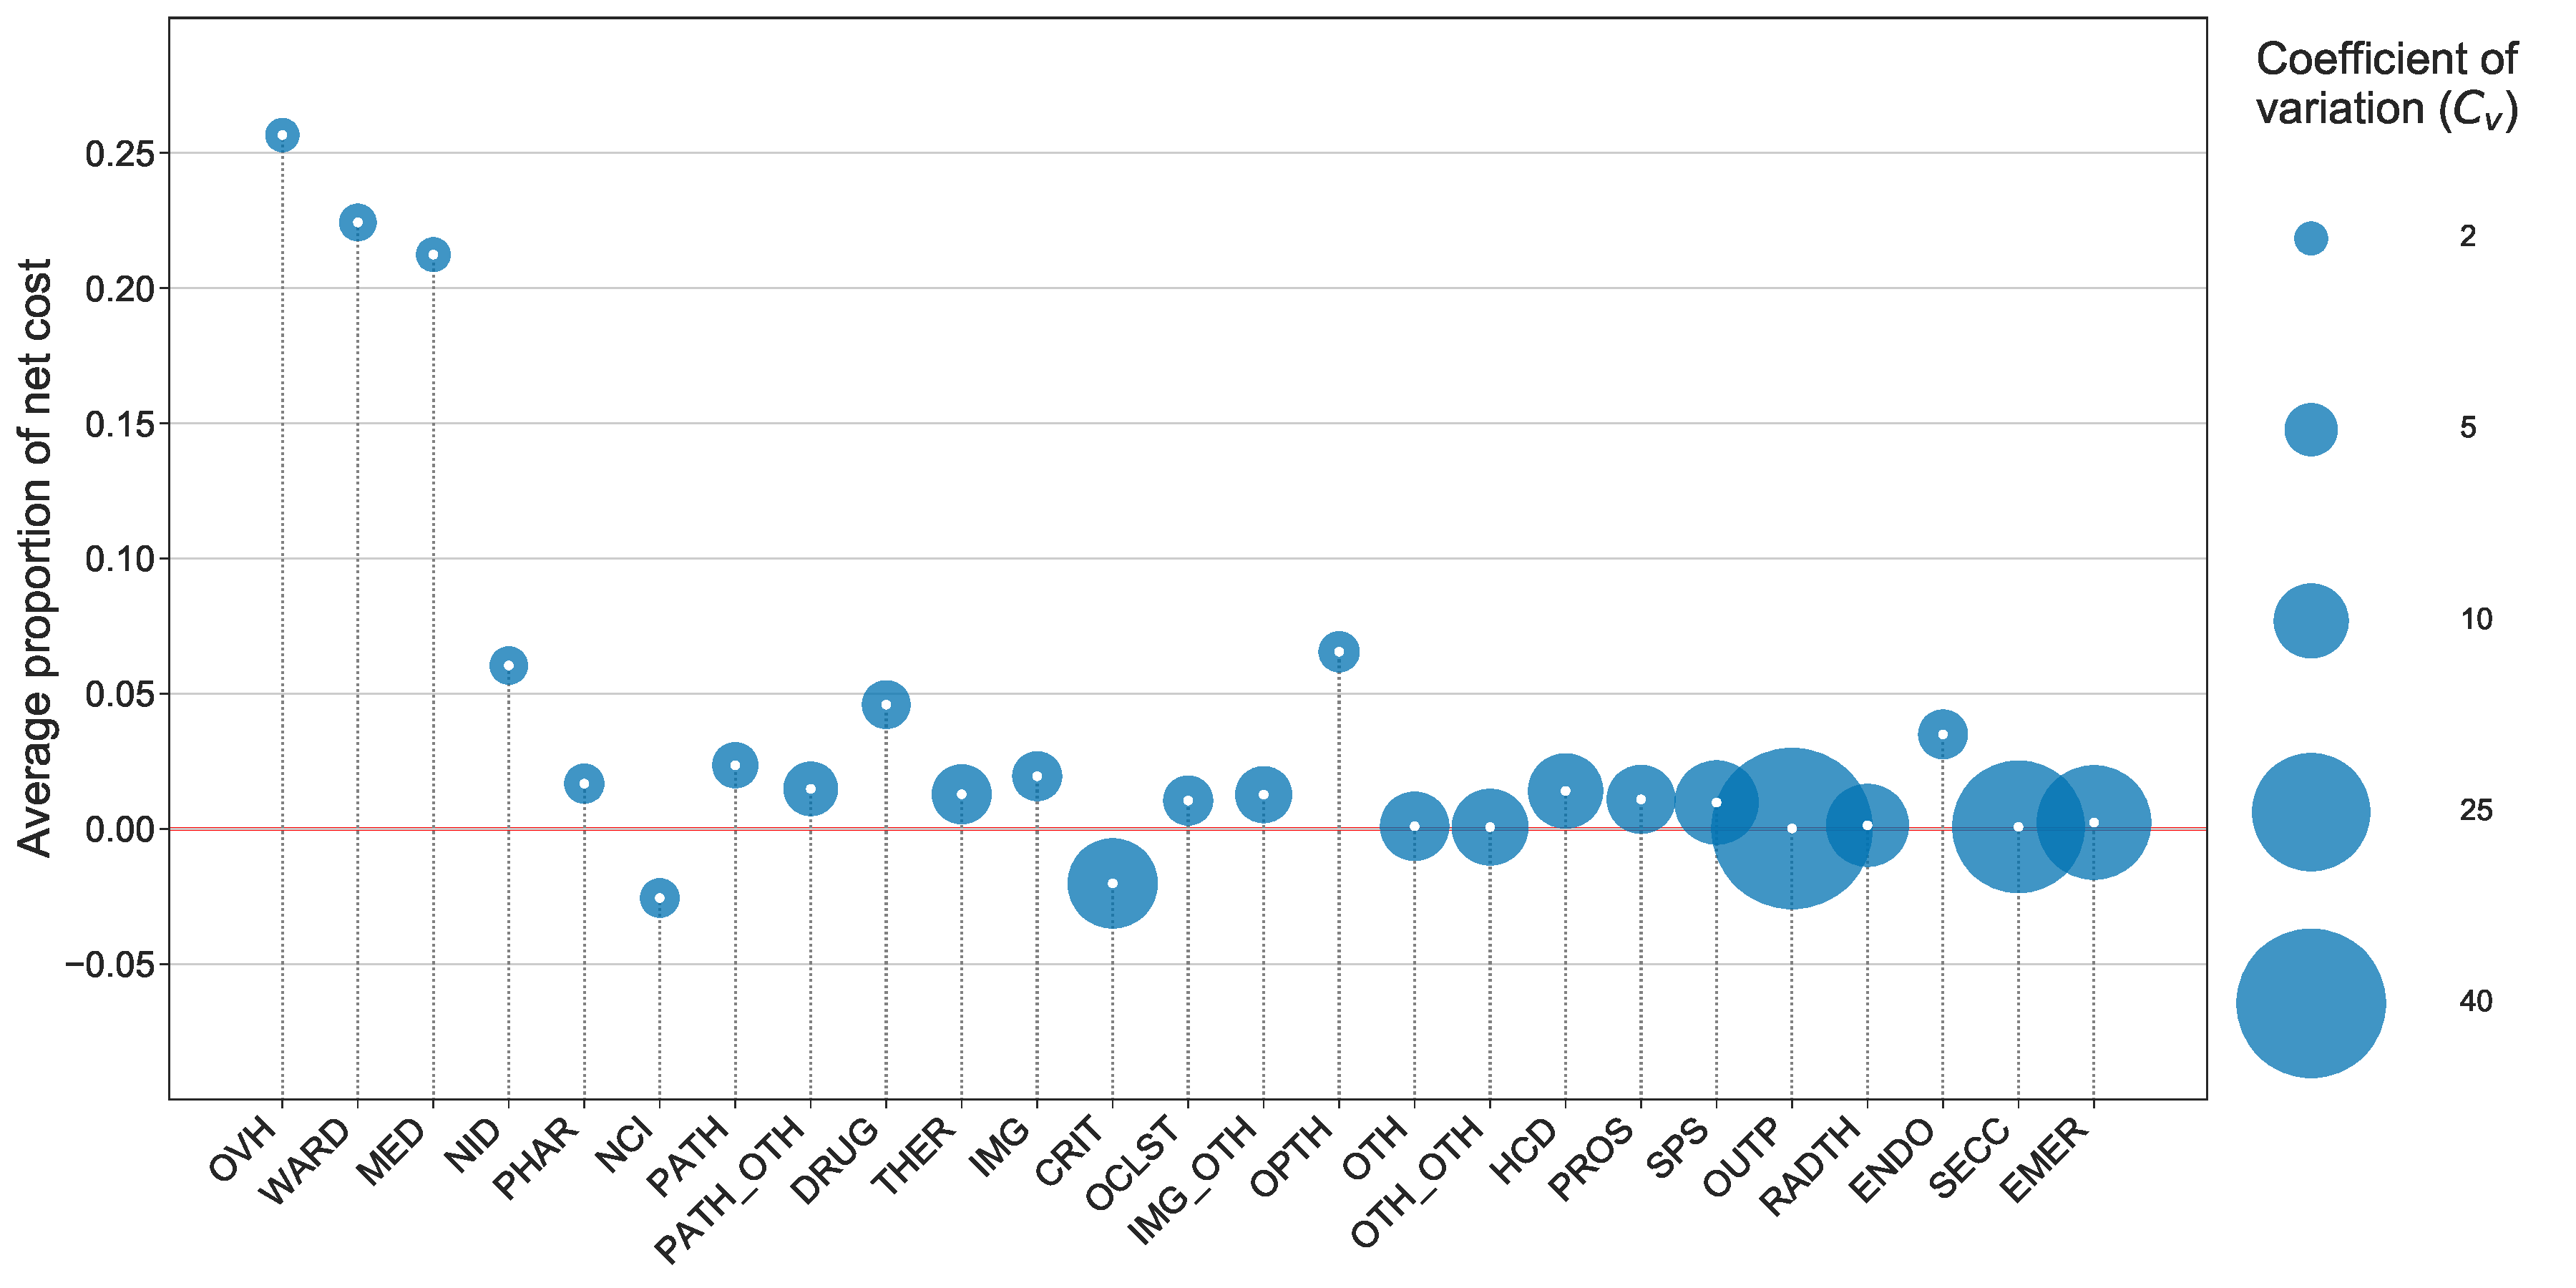
\includegraphics[width=\linewidth]{./img/bubble.pdf}
%    \end{figure}
%}

\section{Why does variation (not) happen?}

\frame{\frametitle{Clustering and partitioning}
    Traditionally:
    \begin{itemize}
        \item Age groupings
        \item Condition-based populations
    \end{itemize}

    A more modern way:
    \begin{itemize}
        \item Clustering of spell-level data
        \item Healthcare utilisation
        \item Pathway mining and similarity
    \end{itemize}
}

\frame{
    \centering
    \huge Thanks for listening!

    @daffidwilde
}

\end{document}
